\documentclass[conference]{IEEEtran-ModifiedForMVIP}
% این فایل از روی نمونه‌ فایل ارائه شده برای کنفرانس مهندسی برق ایران ICEE 
% برای کنفرانس بینایی ماشین و پردازش تصویر ایران به‌روزرسانی شده است.
% فایل منبع و فایلهای ضمیمه‌ی آن با تغییر فایلهایی که توسط آقای دکتر محمود امین طوسی (دانشگاه
% حکیم سبزواری، http://profs.hsu.ac.ir/mamintoosi) در سایت www.parsilatex.com قرار داده 
% شده بودند به دست آمده است. این تغییرات توسط دکتر مسعود بابایی‌زاده داده شده است. 
% البته فایل IEEEtran-ModifiedForICEE.cls در اینجا، 
% اصلاح شده فایل آقای دکتر امین طوسی نیست و مستقیما با دستکاری
% در فایل IEEEtran.cls توسط مسعود بابایی زاده ایجاد شده است.
% برای کنفرانس بینایی ماشین و پردازش تصویر ایران، فایل IEEEtran-ModifiedForICEE.cls 
% با نام IEEEtran-ModifiedForMVIP.cls  تغییر داده شده است.

% مقاله اصلی که این فایل از تغییر فایل آن به دست آمده است، در هفدهمین کنفرانس مهندسی برق 
% ایران در اردیبهشت ۸۸ ارائه شده بوده است.

% شما می‌توانید از این فایل به عنوان یک الگو برای مقالات خود استفاده نمایید.

% برای پردازش پس از یکبار استفاده از xelatex با استفاده از دستور زیر لیست مراجع را تولید نمایید:
% bibtex MVIP_FA_LaTeX_SamplePaper
% و سپس دوبار استفاده از xelatex. 

%%%% فراخوانی پکیج‌های مورد نیاز کاربر %%%%%%%%%%%%%%%%%%%%%%%%%%%%%%%%%%%%%%%%%%%%%%%%%%
\usepackage{setspace}
\usepackage{subfigure}
\usepackage{algorithm}
\usepackage{algorithmic}
\usepackage{graphicx}
\usepackage{amsmath}
\usepackage{amssymb}
\usepackage{booktabs}
\usepackage{pdfpages}
%\usepackage[colorlinks, citecolor=blue]{hyperref}

%%%%%%%%%%%%%%%%%%%%%%%%%%%%%%%%%%%%%%%%%%%%%%%%%%%%%%%%%%%%%%%%%%%%%%%%%%%%%%%%%%%%%%%%
%%%% فراخوانی تنظیمات مورد نیاز کنفرانس مهندسی برق ایران و پکیج زی‌پرشین %%%%%%%%%%%%%%%%
% این فایل از روی نمونه‌ فایل ارائه شده برای کنفرانس مهندسی برق ایران ICEE برای کنفرانس بینایی ماشین و پردازش تصویر ایران به‌روزرسانی شده است.
% این فایل شامل تنظیماتی است که قبل از لود شدن پکیج زی‌پرشین باید انجام شوند.
% نویسنده: مسعود بابایی‌زاده
% نسخه 1.0.0
% تاریخ: ۵ مهرماه ۱۳۹۳
%%%%%%%%%%%%%%%%%%%%%%%%%%%%%%%%%%%%%%%%%%
% Start of Page Setup:
\usepackage[top=25mm, bottom=25mm, left=20mm, right=20mm]{geometry}
\setlength{\columnwidth}{82mm}
\setlength{\columnsep}{6mm}
% End of Page Setup
%%%%%%%%%%%%%%%%%%%%%%%%%%%%%%%%%%%%%%%%%%
% یکی از دو روش زیر را انتخاب کنید. گذاشتن حالت «کشیده» باعث می‌شود که تنطیم
% طول خطها بجای اینکه با کم و زیاد کردن فاصله بین کلمات انجام شود، با کشیدن
% کلمات انجام شود. این حالت در فارسی صحیح‌تر و خیلی زیباتر است (برخلاف انگلیسی که کشیدن کلمات
% در آن معنی ندارد و تنطیم طول خطوط فقط با کم و زیاد کردن فاصله بین کلمات صورت
% می‌گیرد). اما با استفاده از حالت «کشیده»، اگر از Acrobat Adobe برای دیدن خروجی پی‌دی‌اف
% استفاده کنید این کشیده‌ها را می‌بینید که چندان زیبا نیست (در نسخه چاپی وجود ندارند).
% اگر می‌خواهید اینها را نبینید در قسمت  Edit->Preferences->PageDisplay گزینه
% Enhance Thin Lines
% را غیرفعال کنید. اما اگر از SumatraPDF برای دیدن فایل پی‌دی‌اف استفاده می‌کنید، تنظیم خاصی
% نیاز نیست.
\usepackage[Kashida]{xepersian}
% \usepackage{xepersian}
% این فایل از روی نمونه‌ فایل ارائه شده برای کنفرانس مهندسی برق ایران ICEE برای کنفرانس بینایی ماشین و پردازش تصویر ایران به‌روزرسانی شده است.
% این فایل شامل تنظیماتی است که بعد از لود شدن پکیج زی‌پرشین باید انجام شوند.
% نویسنده: مسعود بابایی‌زاده
% نسخه 1.0.0
% تاریخ: ۳ مهرماه ۱۳۹۳

%%%%%%%%%%%%%%%%%%%%%%%%%%%%%%%%%%%%%%%%%%
% Font settings

\settextfont[ BoldFont={XB Kayhan Bd.ttf}, BoldItalicFont={XB Kayhan BdIt.ttf}, ItalicFont={XB Kayhan It.ttf},Scale=1.2]{XB Kayhan.ttf}
\setdigitfont[Scale=1.2]{XB Kayhan.ttf}
\setlatintextfont[Scale=1]{Times New Roman}
\defpersianfont\titlefont[Scale=1]{IRTitr.ttf}
\setiranicfont[Scale=1.2]{XB Kayhan It.ttf}				% ایرانیک، خوابیده به چپ

%%%%%%%%%%%%%%%%%%%%%%%%%%%%%%%%%%%%%%%%%%
% تنظیم فاصله خطوط:
% زیاد کردن \baselineskip بر خلاف \baselinestreatch روی محیط ریاضی تاثیری ندارد. اما \baselineskip را باید بعد از \begin{document} زیاد کرد. با توجه به اینکه singlespace برای فرمولهای ریاضی در متن فارسی زیادی کوچک است،‌ پس برای آنکه طبق اعداد بالا فاصله خطوط در فرمولهای 1 برابر و در متن فارسی 1.1 برابر باشد، لازم است که طبق دستور زیر \baselinestreatch برابر 1 قرار داده شود و سپس درون متن و بعد از  \begin{document} باید \baselineskip را 1.1/1.0=1.1 برابر نمود. یعنی:

\renewcommand{\baselinestretch}{1}
%\setlength{\baselineskip}{1.1\baselineskip}   ->  This is inside the text and right after \begin{document}
%برای آنکه کاربر مجبور نباشد دستور بالا را دستی بعد از begin document اضافه کند، دستورات زیر را می‌نویسیم:
\let\olddocument=\document
\let\endolddocument=\enddocument
\renewenvironment{document}{\begin{olddocument}\setlength{\baselineskip}{1.53\baselineskip}}{\end{olddocument}}
%در اینصورت فاصله فرمولها با متن کمی زیاد می‌شود که آن را نیز با دستورات زیر می‌توان حل کرد:
\let\oldequation=\equation
\let\endoldequation=\endequation
% For Yas font
%\renewenvironment{equation}{\vspace{0.2em}\begin{oldequation}}{\vspace{-0.5em}\end{oldequation}\ignorespacesafterend}
% For IRLotus font
\renewenvironment{equation}{\vspace{0.0em}\begin{oldequation}}{\vspace{-0.4em}\end{oldequation}\ignorespacesafterend}


% هبا اعداد بالا در فهرست مطالب و فهرست اشکال و جداول نیز فاصله خطوط زیاد است. که به صورت زیر می‌توان اصلاح کرد (یعنی برای آنها baselineskip را مجددا به عدد قبلی برگرداند، یعنی در معکوس 1.1 که برابر 0.91 می‌شود ضرب کرد):
\let\oldtableofcontents=\tableofcontents
\renewcommand{\tableofcontents}{\begingroup\setlength{\baselineskip}{0.91\baselineskip}\oldtableofcontents\endgroup}

\let\oldlistoffigures=\listoffigures
\renewcommand{\listoffigures}{\begingroup\setlength{\baselineskip}{0.91\baselineskip}\oldlistoffigures\endgroup}

\let\oldlistoftables=\listoftables
\renewcommand{\listoftables}{\begingroup\setlength{\baselineskip}{0.91\baselineskip}\oldlistoftables\endgroup}

% دستور با اعداد بالا، فاصله خطوط در یک متن انگلیسی زیادی  (مثلا فهرست مراجع) بزرگ است. در پایین با تغییر تعریف latin آن را در 0.91 ضرب کرده‌ام:
\let\oldlatin=\latin
\let\endoldlatin=\endlatin
\renewenvironment{latin}{\begin{oldlatin}\setlength{\baselineskip}{0.91\baselineskip}}{\end{oldlatin}}

%%%%%%%%%%%%%%%%%%%%%%%%%%%%%%%%%%%%%%%%%%
% دستور زیر برای زیادکردن تورفتگی اول هر پاراگراف است. مقدار پیش‌فرض قبلی، برای متون انگلیسی است و برای متون فارسی زیادی کوچک است.

\parindent=1cm

%%%%%%%%%%%%%%%%%%%%%%%%%%%%%%%%%%%%%%%%%%
% برای آنکه در شماره‌گذاری حرفی و ابجد به جای آ از الف استفاده شود (این دستورات از تمپلیت تهیه شده توسط دکتر امین‌طوسی برا پایان‌نامه‌های دانشگاه حکیم سبزواری برداشته شده است):

\makeatletter

 \def\abj@num@i#1{%
   \ifcase#1\or الف\or ب\or ج\or د%
            \or ه‍\or و\or ز\or ح\or ط\fi
   \ifnum#1=\z@\abjad@zero\fi}   
  
   \def\@harfi#1{\ifcase#1\or الف\or ب\or پ\or ت\or ث\or
 ج\or چ\or ح\or خ\or د\or ذ\or ر\or ز\or ژ\or س\or ش\or ص\or ض\or ط\or ظ\or ع\or غ\or
 ف\or ق\or ک\or گ\or ل\or م\or ن\or و\or ه\or ی\else\@ctrerr\fi}
 
 \makeatother



%%%%%%%%%%%%%%%%%%%%%%%%%%%%%%%%%%%%%%%%%%%%%%%%%%%%%%%%%%%%%%%%%%%%%%%%%%%%%%%%%%%%%%%%
% تعریف دستورات جدید مورد نیاز کاربر %%%%%%%%%%%%%%%%%%%%%%%%%%%%%%%%%%%%%%%%%%%%%%%%%%%
\newcommand\femph[1]{\lr{''}#1\lr{``}}
\newcommand{\SR}{وضوحِ برتر}%{\textiranic{ وضوحِ برتر }}
\newcommand{\HR}{وضوح بالا}
\newcommand{\registration}{ثبت تصویر}
\newcommand{\fusion}{آمیختن}
\newcommand{\fused}{آمیخته}

\newcommand{\warp}{\mathbf{W}(\mathbf{x};\mathbf{p})}
\newcommand{\IWarp}{I(\mathbf{W}(\mathbf{x};\mathbf{p}))}
\newcommand{\round}[2]{\frac{\partial{#1}}{\partial{#2}}}
\newcommand{\roundB}[2]{\frac{\partial{\mathbf{#1}}}{\partial{\mathbf{#2}}}}


% شروع متن اصلی %%%%%%%%%%%%%%%%%%%%%%%%%%%%%%%%%%
\begin{document}
% دستور زیر باعث امکان استفاده از \thanks می‌شود.
\IEEEoverridecommandlockouts 

\title{
طراحی و پیاده‌سازی ضرب‌کنندهٔ ماتریس توسط Verilog
}

\author{
\IEEEauthorblockN{
احمد سلیمی
\textsuperscript{1}،
کیمیا نوربخش
\textsuperscript{1}،
ساعی سعادت
\textsuperscript{1}،
علیرضا حسین‌پور
\textsuperscript{1}
}
\IEEEauthorblockA{\textsuperscript{1}
دانشگاه صنعتی شریف، دانشکده مهندسی کامپیوتر}
}

%\date{}
\maketitle
% چکیده مقاله
\begin{abstract}
\end{abstract}
\begin{IEEEkeywords}
% کلمات کلیدی
\end{IEEEkeywords}

%\IEEEpeerreviewmaketitle

\section{مقدمه}


\section{معماری سیستم}

معماری این سیستم، از سه لایهٔ اصلی تشکلی شده‌است. در ادامه، معماری و جزئیات هر یک از این لایه‌ها، توضیح داده شده است.
\\
برای ارتباط بین تمامی ماژول‌ها، برای اطمینان از این که ورودی و خروجی‌ها هنگام استفاده شدن تغییر نمی‌کنند و مقدار صحیحی دارند، برای هر کدام دو سیگنال stable و acknowledge در نظر می‌گیریم.
نحوه‌ی استفاده از آن‌ها بدین گونه است که ماژولی که مقدار را دارد و می‌خواهد آن‌را پاس بدهد، با استفاده از سیگنال stable به ماژول گیرنده اعلام می‌کند که ورودی آماده‌ی استفاده است،
 سپس ماژول گیرنده با استفاده از سیگنال acknowledge اعلام می‌کند که ورودی را با موفقیت دریافت کرده و ماژول فرستنده می‌تواند آن را تغییر دهد.

\subsection{
    ضرب‌کنندهٔ ماتریس ترتیبی
}

در این ماژول مانند ضرب ماتریسی عادی، دو ماتریس 
$m \times m$
را در هم ضرب می‌کنیم. می‌دانیم که برای به دست آوردن درایه 
$ij$
حاصلضرب، باید سطر $i$ ام ماتریس اول را در ستون $j$ ام ماتریس دوم ضرب کنیم. برای این موضوع به ازای هر 
$1\leq i\leq m , 1\leq j\leq m $،
داریم:
$$R_{ij} = \sum_{k=0}^m{A_{ik} \times B_{kj}}،$$
که در آن،
$R$
ماتریس
$m \times m$
حاصل‌ضرب است.\\
در این ماژول برای محاسبه جمع و ضرب‌ها، از ماژول‌های جمع‌کننده و ضرب‌کننده اعشاری
\LTRfootnote{\lr{floatng point adder and multiplier}} 
 استفاده می‌کنیم.\\
ماژول ضرب‌کنندهٔ ماتریس ترتیبی
\LTRfootnote{\lr{sequential matrix multiplier}} 
 این فرایند را در قالب یک ماشین حالت انجام می‌دهد. برای محاسبه درایه $i,j$ ام، یک 
 \lr{accumulator}
 برای نگه‌داری جواب نهایی در نظر می‌گیریم و سپس
  به ازای هر $k$، ابتدا با استفاده از ماژول 
 \lr{FP\_multiplier} 
  حاصل
$A_{ik}\times B_{kj}$
 را محاسبه می‌کنیم و با استفاده از ماژول
  \lr{FP\_Adder}
 ، به ازای $k$ های مختلف جواب را آپدیت می‌کنیم.  

شکل
\ref{fig:SequentialBD}
بلوک دیاگرام ضرب‌کنندهٔ ماتریس ترتیبی را نشان می‌دهد.
باید توجه کرد که حافظه‌ای که حاوی ماتریس‌های ورودی و ماتریس جواب است، در خارج این ماژول قرار دارد.
در نتیجه، واحد کنترل در این ماشین حالت محدود
\LTRfootnote{Finite State Machine}
اندیس‌های درایه‌های موردنیاز خود، یعنی
$a_i, a_j, b_i, b_j, z_i, z_j$
را تعیین می‌کند، و مقادیر مربوط به هر درایه در ماتریس‌های ورودی در
$a_{in}$
و
$b_{in}$
قراره گرفته، و مقدار
$z_{out}$
نیز در ماتریس جواب قرار داده‌می‌شود.

\begin{figure}[t]
\centering 
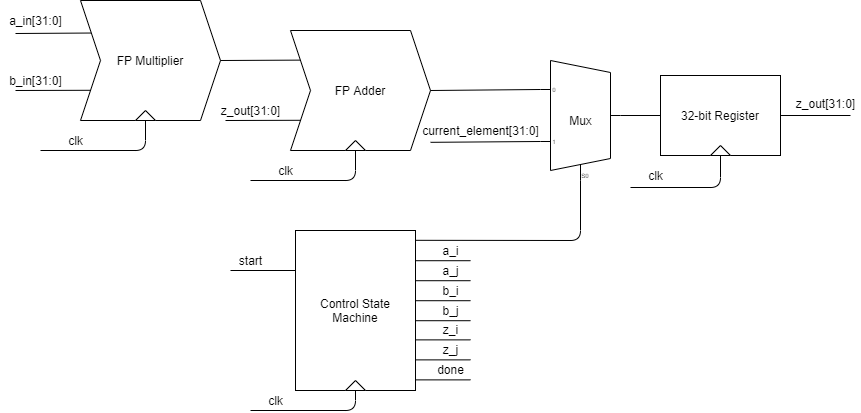
\includegraphics[width=1\linewidth]{Images/SequentialBD.png}
\caption{
\centering
بلوک دیاگرام ضرب‌کنندهٔ ماتریس ترتیبی.
}\label{fig:SequentialBD}
\end{figure}

\subsection{
    ضرب‌کنندهٔ ماتریس سطری در ستونی
}

وظیفهٔ این ماژول، این است که با استفاده از یک ماژول ضرب‌کنندهٔ ماتریس ترتیبی، حاصل‌ضرب یک ماتریس سطری
$m \times n$
در یک ماتریس ستونی
$n \times m$
را محاسبه‌کند.
حاصل این ضرب، یک ماتریس
$m \times m$
خواهد بود.
\\
برای انجام این‌ کار، ابتدا ماتریس 
$m \times n$
خود را به 
${\lceil\frac{n}{m}\rceil}$
تا ماتریس 
$m \times m$
کنار هم تقسیم‌بندی می‌کنیم.
مشابها ماتریس 
$n \times m$
خود را نیز به 
$\lceil\frac{n}{m}\rceil$
تا ماتریس 
$m \times m$
بالای هم تقسیم‌بندی می‌کنیم.
حال با استفاده از ماژول ضرب‌کننده ماتریس ترتیبی و با توجه به  این که قاعده ضرب بلوکی در ماتریس‌ها برقرار است، هر یک از این ماتیس‌های 
$m \times m$
را به مانند یک عدد در نظر می‌گیریم و ماتریس‌های متناظر را در هم ضرب می‌کنیم.

\begin{figure}[t]
\centering 
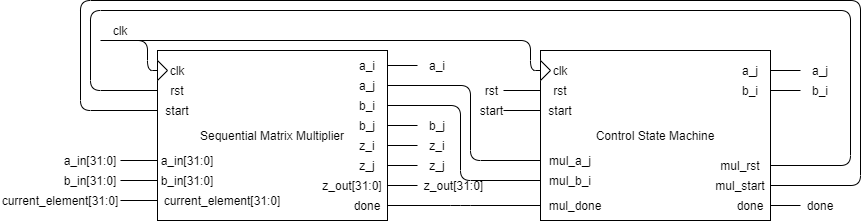
\includegraphics[width=1\linewidth]{Images/RowColBD.png}
\caption{
\centering
بلوک دیاگرام ضرب‌کنندهٔ ماتریس سطری در ستونی.
}\label{fig:SequentialBD}
\end{figure}


\subsection{
    ضرب‌کنندهٔ ماتریس موازی
}

\section{شبیه‌سازی و نتایج}

\section{سنتز و نتایج}

\section{نتیجه‌گیری}


%\begin{table}[ht]
%\centering
%\caption{پارامتر‌های روش‌های دسته‌بندی.}
%\begin{tabular}[t]{ c c }
%\toprule
%روش دسته‌بندی & تعریف پارامترها\\
%\midrule
%\lr{KNN} & 
%\begin{tabular}{r l}
%تعداد نزدیک‌ترین همسایه‌ها & 3
%\end{tabular}\\
%\midrule
%بیز ساده‌انگارانه & -------\\
%\midrule
%انتشار رو به عقب &
%\begin{tabular}{r l}
%تعداد نورون لایهٔ نهان & 10\\
%نرخ یادگیری &
%$0.3$\\
%تعداد تکرار & 1000
%\end{tabular}\\
%\midrule
%\lr{NTC} &
%\begin{tabular}{r c l}
%نرخ یادگیری &
%\hspace{1cm}
%&‌$0.3$\\
%تعداد تکرار &
%\hspace{1cm}
%& 100
%\end{tabular}
%\end{tabular}
%\label{tab:NTCHyperParams}
%\end{table}

در صورتی که مقدار $n$ بر $m$ بخش پذیر نباشد، 
ماتریس را به جای 
$n \times n$ ،
$ \lceil \frac{n}{m} \rceil \times m$
در نظر می‌گیریم و درایه‌های اضافی را با $0$ پر می‌کنیم.
در نظر می‌گیریم و درایه‌های اضافی را با $0$  پر می‌کنیم
در نهایت برای ذخیره کردن جواب اندیس‌ها از $n$ فراتر نخواهند رفت در نتیجه جواب $n \times n$ باقی خواهد ماند.

\newpage
‌
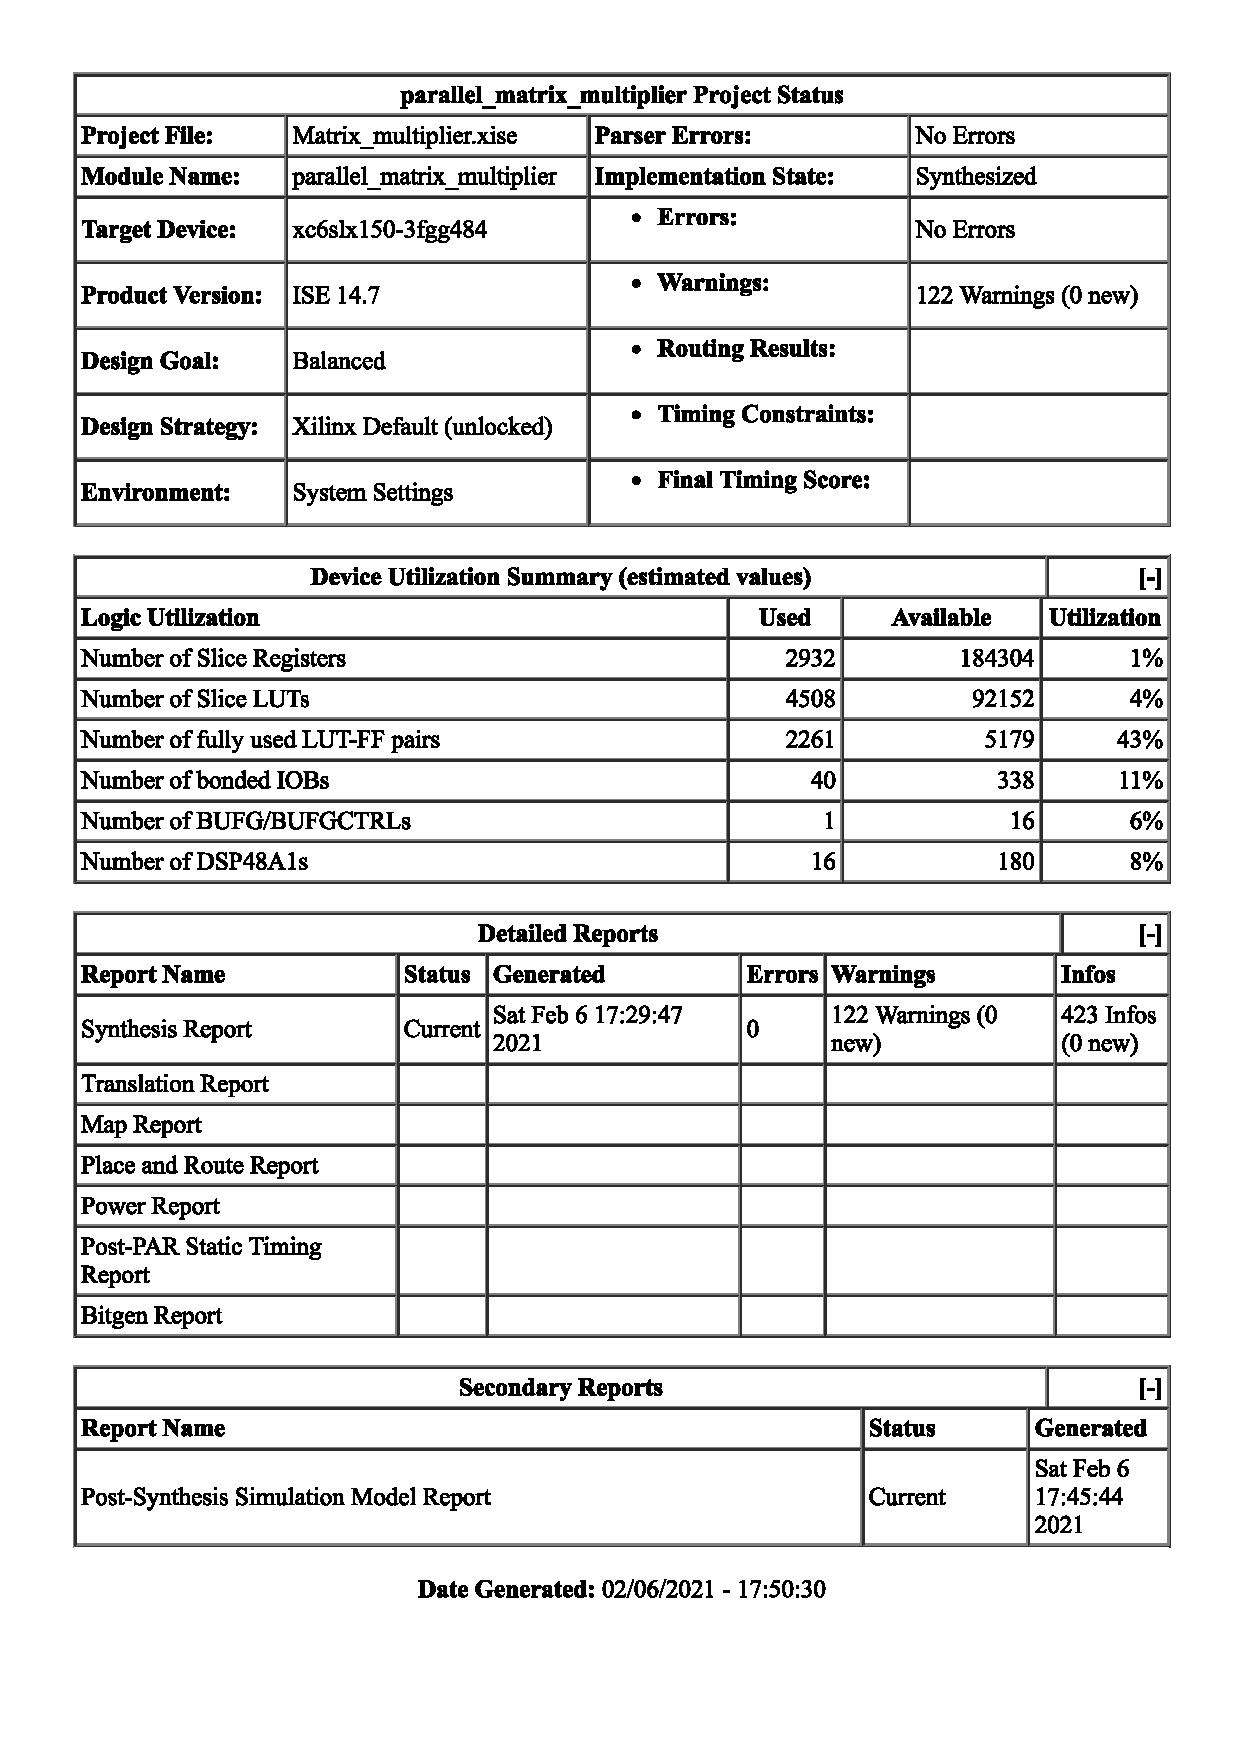
\includepdf[pages=-]{ParallelSummary.pdf}

\end{document}